\chapter{Case Study 1: Shut the Box}
\label{cs1}

\section{Game description (1/2 page)}
\label{cs1:stb_description}
Shut the Box is a single player game, where the player aims to cover as many boards as possible through a series of dice rolls. The game starts with a series of \emph{boards}, each numbered sequentially starting from 1, with each board originally uncovered. Each round, the player rolls a set of dice. The player must then cover a set of uncovered boards whose sum is equal to the sum of the dice. For instance, if the player rolls a 1 and a 2, then the player must either cover boards 1 and 2, or cover board 3. The game proceeds in this manner until the player cannot cover a suitable set of uncovered boards. A player's \emph{score} for a round of Shut the Box is defined as the sum of all covered boards.

Throughout the case study, unless otherwise stated, we consider the variant of Shut the Box where there are 12 boards, and the player rolls two six-sided dice each round.

When playing Shut the Box, it soon becomes clear that some configurations of boards are highly desirable, while others are more challenging. For instance, consider the situation in Figure \ref{cs1:cover_choice}, where 4 boards are remaining and a 7 is rolled. Two possible coverings are available, but leaving boards 1 and 2 uncovered is more valuable than leaving board 3 uncovered - in particular, if a 3 is rolled then every board can be covered in both cases, but if a 2 is rolled then board 2 may be covered in the former case, while no valid covering exists in the latter case. Hence covering boards 3 and 4 leads to a higher expected score at the end of the game than covering boards 1, 2 and 4.

\begin{figure}
\label{cs1:cover_choice}
    \centering
    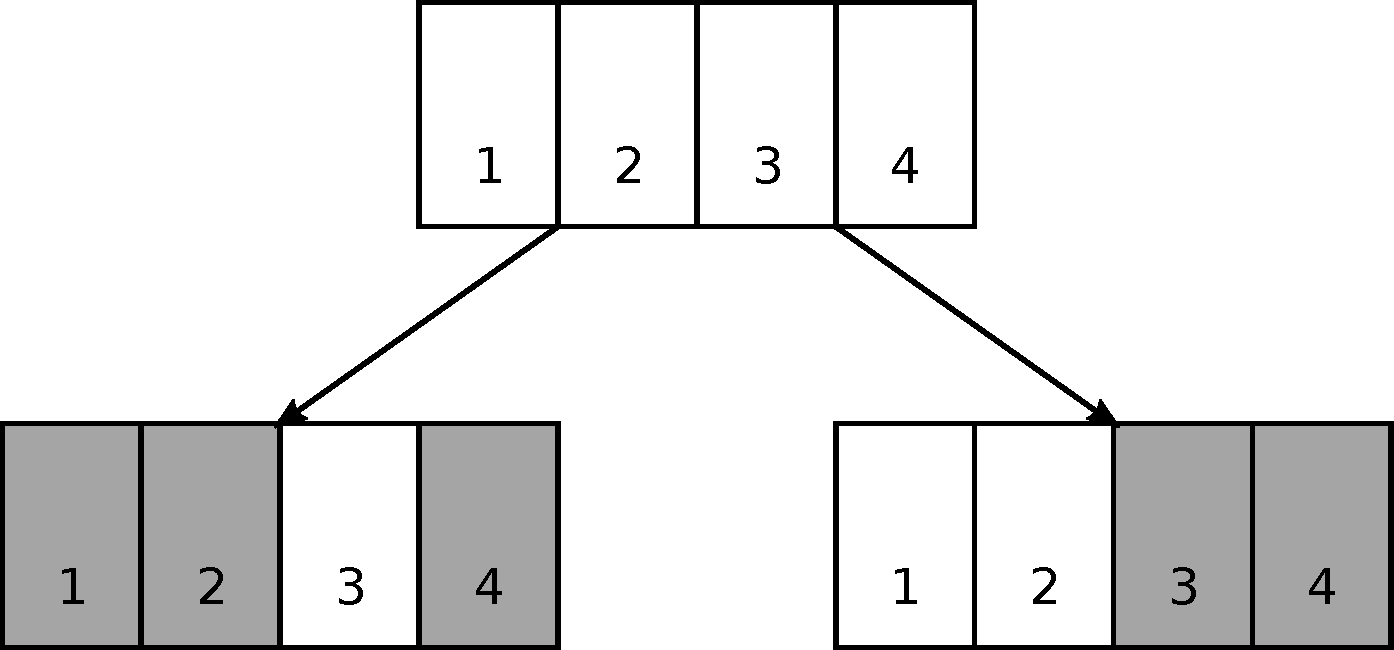
\includegraphics[width=0.5\linewidth]{images/cover_choice.pdf}
    \caption{When boards 1 to 4 are all uncovered, and a 7 is rolled, there are two possible valid coverings - covering boards 1, 2 and 4 (on the left), and covering boards 3 and 4 (on the right).}
\end{figure}

Intuitively, this suggests that lower numbered boards are more valuable later in the game, since they increase the set of possible die rolls that a player can roll without ending the game. From this intuition, we develop two potential strategies for playing Shut the Box. The \emph{high-board strategy} is the strategy where the player always elects to cover the highest number board at each stage, while the \emph{low-board strategy} is the converse, where the player always elects to cover the lowest numbered boards at each stage.

When evaluating the effectiveness of these strategies, model checking is a suitable strategy. Since these strategies are deterministic, we may define DTMCs that model Shut the Box under these strategies, define the score of the game as a reward structure, and evaluate the expected score when the game terminates. However, we are also interested in the \emph{optimal} strategy - that is, the strategy which maximises the expected score of Shut the Box. Trying to enumerate and consider every possible strategy would be challenging, both conceptually and computationally. Instead, we consider the case where \emph{no} strategy is defined - in other words, an entirely nondeterministic strategy. In order to achieve this, we consider a generalisation of a DTMC.

\section{Background}
\label{cs1:stb_background}

We start by introducing Markov decision processes (MDPs), which are generalisations of DTMCs allowing for actions to be taken at each state, each leading to different probabilistic transitions between states. We then consider adversaries - resolutions of nondeterministic choice in MDPs - then briefly discuss how optimal adversaries are computed.

\subsection{Markov decision processes}
\label{cs1:mdps}
First, we define an MDP as a modification of a DTMC.

\begin{definition}
\label{cs1:def_mdps}

A Markov decision process (MDP) is a tuple $(S, \bar{s}, \mathbf{Steps}, L)$, where $S$, $\bar{s}$ and $L$ have the same meanings as in Definition \ref{back:dtmc}. $\mathbf{Steps} : S \rightarrow 2^{Act \times Dist(S)}$ is the new transition probability function, where states are mapped to a set of pairs of actions and discrete probability distributions, where $Act$ represents the set of actions the player can take.

\end{definition}

For example, in a game of Shut the Box, $Act$ is the set of possible subsets of boards that the player can cover (such as the action of covering boards 3 and 5 simultaneously). Hence, $\mathbf{Steps}$ maps each state, including the current die value and the current set of uncovered boards, to the set of all possible covering arrangements along with the associated state transition.

Note here that, in general, a state may be associated to more than one action-distribution pair. Indeed, this is where nondeterminism is introduced into the MDP. In order to resolve this nondeterminism, we introduce the concept of adversaries.

\begin{definition}
\label{cs1:adversaries}

Given a \emph{finite} path $\omega = s_0 \rightarrow s_1 \rightarrow \dots \rightarrow s_n$, an adversary is a function $\sigma$ which maps each finite path to an action-distribution pair, more specifically an element of $\mathbf{Steps(s_n)}$.

\end{definition}

A key remark on this definition is that adversaries make decisions depending on the entire execution history up to a state $s_n$, not just the state $s_n$ itself. However, we primarily consider $memoryless adversaries$, where the adversary always picks the same choice in a given state. In particular, this adversary can be viewed as a map from states to action-distribution pairs, as opposed to a map from finite paths to action-distribution pairs. Throughout the remainder of the dissertation, we only consider memoryless adversaries unless stated otherwise.

When an MDP is considered under an adversary, nondeterministic choice is resolved, and a DTMC is obtained. Hence, under a specific adversary, we can apply the model checking techniques introduced in Section \ref{back:prob_mod_check} to evaluate properties of an MDP.

\section{Analysis (3 pages)}

Collect some data, show the results.

\hrule

\Blindtext

\Blindtext

\Blindtext

\section{Evaluation(2 pages)}

The key section - use the results from model checking to answer questions about the game (for instance, to examine the difficulty and/or complexity of a game).

\hrule

\Blindtext

\Blindtext